\documentclass[twocolumn]{article}
\usepackage{fancyhdr}
\usepackage{floatrow} \floatsetup[table]{font={footnotesize,sf}} % Small table text.
\usepackage{hyperref}
\usepackage{datetime}
\usepackage[left=1in, right=1in, top=1in, bottom=1in]{geometry}
\usepackage{graphicx}
\usepackage{natbib}
\usepackage{pdfpages}
\usepackage{sectsty}
\usepackage{titling}
\bibliographystyle{abbrvnat}

[-IMPORTS-]

\renewcommand{\include}{\input} % Avoid page breaks between sections.

% colors for hyperlinks
\hypersetup{colorlinks=true, allcolors=blue}

\title{[-doc.title-]}

\author{Keegan Trujillo-Green}

\pagestyle{fancy}
\fancyhead[L]{\sf \thetitle}
\fancyhead[R]{\sf \theauthor}
\fancyfoot[C]{\sf \thepage}

\setcounter{secnumdepth}{0}
\allsectionsfont{\raggedright \sf}

\begin{document}

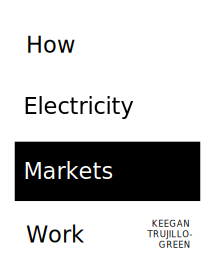
\includepdf{/Users/keegan_green/workspace/src/ontario_electricity_market/cover/cover.pdf}

\newcommand{\documentnote}[1]{{
  \let \thempfn \relax
  \footnotetext[0]{#1}
}}
\documentnote{Cover image: Grid infrastructure spanning Michigan, Ontario, and New York state, copyright OpenStreetMap and Open Infrastructure Map (\url{https://www.openstreetmap.org/copyright}, \url{https://openinframap.org/copyright}).}
\documentnote{This article is available online at: \url{keeganmjgreen.github.io/ontario_electricity_market/}}

[-CONTENT-]

[# if doc.bibliography #]
\begin{flushleft}
\bibliography{[- doc.bibliography | join(", ") -]}
\end{flushleft}
[# endif #]

\end{document}
